\documentclass[10pt,aspectratio=169]{beamer}
\usepackage{poly}

% Optional but useful packages
\usepackage{graphicx}
\usepackage{booktabs}
\usepackage{tikz}

% ================================================================================
% Metadata
% ================================================================================
\title{BarrierNet: Learning Safe Robot Control with Differentiable CBFs}
\subtitle{ELC6011 Assessment 1: Effective introduction to a research paper}
\author{Yufa You}
\institute[AAE]{Department of Aeronautical and Aviation Engineering}
\date{\today}

% ================================================================================
% Main Body
% ================================================================================
\begin{document}
\maketitle

% ------------------------------------------------------------------------------
% 1) Brief topic introduction
% ------------------------------------------------------------------------------
\section{1. Research Topic}

\begin{frame}{1) Research topic: Safe learning-based robot control}
\begin{itemize}
  \item Many robots now use \textbf{learned controllers} (e.g., from demonstrations or end-to-end learning).
  \item In some safety-critical scenarios (e.g., driving), a bad action is \textbf{unacceptable}.
  \item However, learned policies can fail in \textbf{new or unseen situations}.
  \item Research topic: combine \textbf{learning} with \textbf{formal safety guarantees}.
\end{itemize}

\vspace{6pt}
\small
\textit{Intuition: add an ``invisible safety shield'' around a neural controller.}
\end{frame}

% ------------------------------------------------------------------------------
% 2) Critical related literature -> gap
% ------------------------------------------------------------------------------
\section{2. Related Literature \& Research Gap}

\begin{frame}{2) Related literature: common ways}
\begin{itemize}[<+->]
  \item \textbf{Model-based planning/control with guarantees} (e.g., MPC, reachability):
  \begin{itemize}
    \item Strong theory, but often \textbf{computationally heavy} and \textbf{sensitive to modeling/tuning}.
  \end{itemize}
  \item \textbf{Control Barrier Functions (CBFs)}:
  \begin{itemize}
    \item Enforce safety via constraints by solving a small optimization each step,
    \item but constraint design is typically \textbf{hand-crafted} and can be \textbf{conservative}.
  \end{itemize}
  \item \textbf{High-order CBFs} for realistic dynamics:
  \begin{itemize}
    \item More expressive, yet conservatism and feasibility issues often remain in practice.
  \end{itemize}
  \item \textbf{Differentiable optimization layers}:
  \begin{itemize}
    \item End-to-end training is possible, but safety constraints are still usually \textbf{not learned/adaptive}.
  \end{itemize}
\end{itemize}
\end{frame}

\begin{frame}{2) Research gap}
\begin{block}{Key limitation (logical consequence of prior work)}
Classical CBF filters rely on \textbf{fixed, hand-designed} constraints/parameters, which often leads to:
\begin{itemize}
  \item \textbf{Too strict} $\rightarrow$ safe but overly conservative (poor task performance), or
  \item \textbf{Too loose} $\rightarrow$ better performance but may violate safety or become infeasible (e.g., under input limits).
\end{itemize}
\end{block}

\vspace{4pt}
\begin{itemize}
  \item Gap: we need safety constraints that are \textbf{data-adaptive} \emph{while preserving} \textbf{formal safety guarantees}.
\end{itemize}
\end{frame}

% ------------------------------------------------------------------------------
% 3) Clear research aim
% ------------------------------------------------------------------------------
\section{3. Research Aim}

\begin{frame}{3) Research aim}
\begin{block}{Aim of the paper}
Develop an \textbf{end-to-end trainable} safety module that:
\begin{itemize}
  \item can be \textbf{plugged into} a neural controller (as a safety ``filter''),
  \item \textbf{guarantees safety} (e.g., collision avoidance),
  \item and reduces conservatism by \textbf{learning how safety constraints should adapt} to the environment.
\end{itemize}
\end{block}

\begin{itemize}
  \item The proposed approach is called \textbf{BarrierNet}.
\end{itemize}
\end{frame}

% ------------------------------------------------------------------------------
% Visual summary: What does the paper do and how well does it work?
% ------------------------------------------------------------------------------


\begin{frame}{Research aim}

\begin{columns}

    % ---------------- LEFT COLUMN ----------------
    \begin{column}{0.48\textwidth}
        \centering
        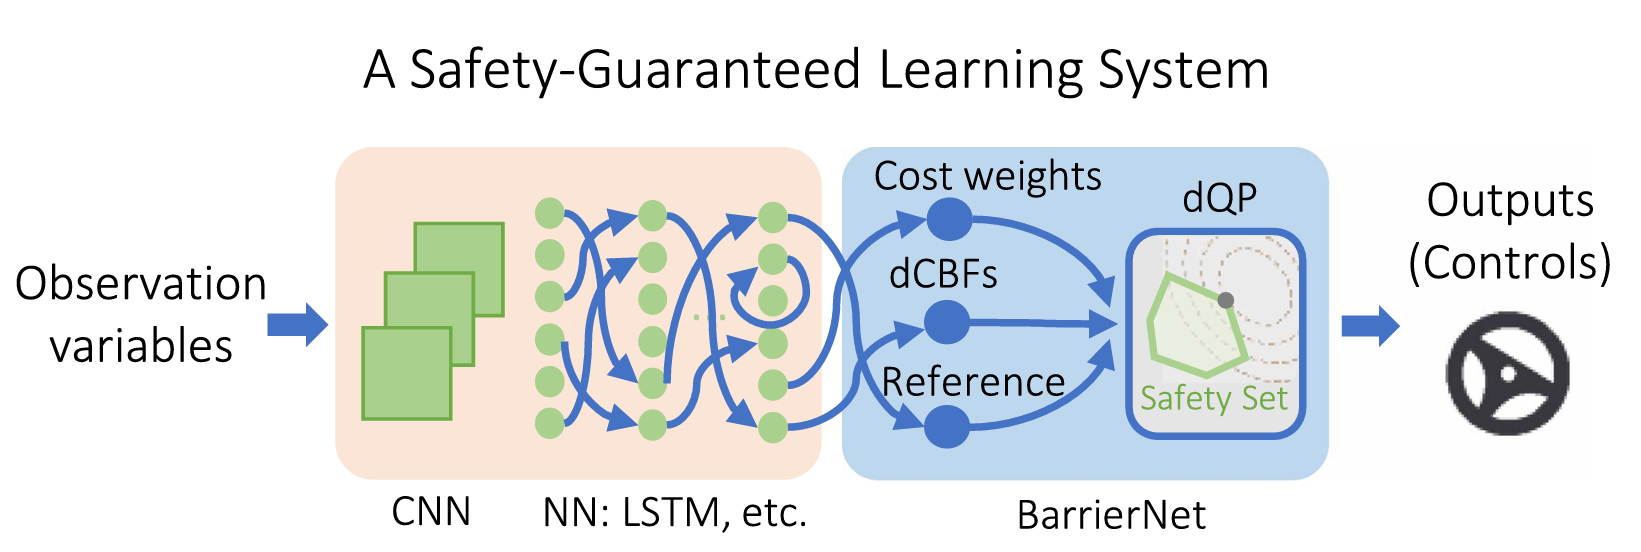
\includegraphics[width=\linewidth]{fig1}
        
        \vspace{4pt}
        \small
        \textbf{Fig.1: Method overview}
        
        \vspace{4pt}
        \footnotesize
        Neural controller + differentiable CBF-QP layer  
        $\rightarrow$ safe action with formal guarantees
    \end{column}

    % ---------------- RIGHT COLUMN ----------------
    \begin{column}{0.40\textwidth}
        \centering
        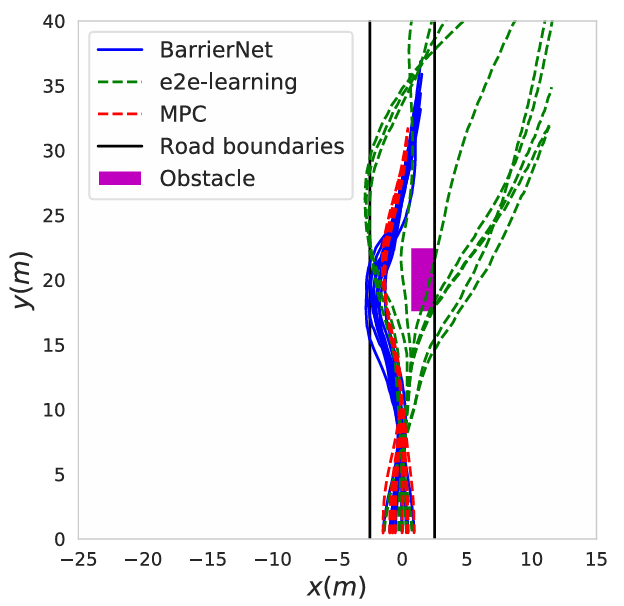
\includegraphics[width=\linewidth]{fig16}
        
        \vspace{4pt}
        \small
        \textbf{Fig.16: Experimental results}
        
        \vspace{4pt}
        \footnotesize
        Adaptive safety constraints  
        $\rightarrow$ safer behavior with less conservatism
    \end{column}

\end{columns}

\vspace{6pt}
\small
\textit{Take-home message: BarrierNet keeps formal safety guarantees while improving real-world performance.}

\end{frame}


\backmatter
\end{document}


\begin{figure}
    \centering
    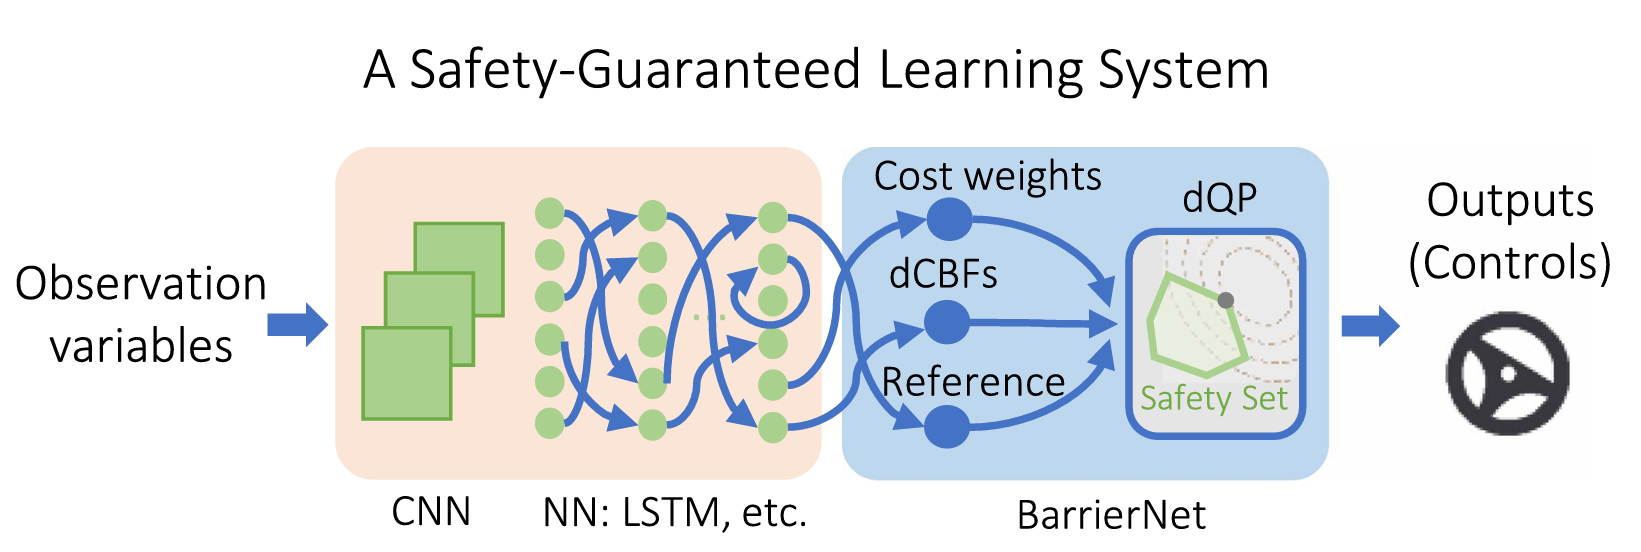
\includegraphics[width=0.5\linewidth]{fig1.png}
    \caption{Enter Caption}
    \label{fig:placeholder}
\end{figure}